%%%%%%%%%%%%%%%%%%%%%%%%%%%%%%%%%%%%%%%%%
% Beamer Presentation
% LaTeX Template
% Version 1.0 (10/11/12)
%
% This template has been downloaded from:
% http://www.LaTeXTemplates.com
%
% License:
% CC BY-NC-SA 3.0 (http://creativecommons.org/licenses/by-nc-sa/3.0/)
%
%%%%%%%%%%%%%%%%%%%%%%%%%%%%%%%%%%%%%%%%%

%----------------------------------------------------------------------------------------
%	PACKAGES AND THEMES
%----------------------------------------------------------------------------------------

\documentclass{beamer}

\newcommand{\EMSE}{ {\rm EMSE}}
\newcommand{\CC}{ {\rm CC}}
\newcommand{\MSE}{ {\rm MSE}}
\newcommand{\WIN}{\scriptscriptstyle {\rm WIE}}
\newcommand{\OROI}{\scriptscriptstyle {\rm out ROI}}
\newcommand{\Her}{\scriptscriptstyle H}
\newcommand{\T}{\scriptscriptstyle T}
\newcommand{\LMS}{\scriptscriptstyle {\rm LMS}}
\newcommand{\RDE}{\scriptscriptstyle {\rm RDE}}
\newcommand{\MRD}{\scriptscriptstyle {\rm MRD}}
\newcommand{\MSD}{\scriptscriptstyle {\rm MSD}}
\newcommand{\SBD}{\scriptscriptstyle {\rm SBD}}
\newcommand{\SDD}{\scriptscriptstyle {\rm SDD}}
\newcommand{\WIE}{\scriptscriptstyle {\rm WIE}}
\newcommand{\R}{\scriptscriptstyle {\rm R}}
\newcommand{\I}{\scriptscriptstyle {\rm I}}
\newcommand{\mT}{\scriptscriptstyle -T}
\newcommand{\vir}{,\hspace{-0.15ex}}
\newcommand{\M}{\scriptscriptstyle M}
\newcommand{\MMA}{\rm \scriptscriptstyle MMA}
\newcommand{\neigh}{\scriptscriptstyle {\rm neigh}}
\newcommand{\st}{\scriptscriptstyle {\rm st}}
\newcommand{\nd}{\scriptscriptstyle {\rm nd}}
\newcommand{\CSD}{\scriptscriptstyle {\rm CSD}}
\newcommand{\E}{{\rm E}}
\newcommand{\uM}{{\mathbf u}}
\newcommand{\rM}{{\mathbf r}}
\newcommand{\xM}{{\mathbf x}}
\newcommand{\yM}{{\mathbf y}}
\newcommand{\XM}{{\mathbf X}}
\newcommand{\w}{{\mathbf w}}
\newcommand{\wo}{{\mathbf{w}}_{\rm o}}
\newcommand{\q}{{\mathbf q}}
\newcommand{\qp}{{\mathbf {\dot{q}}}}
\newcommand{\Nuquad}{\|{\mathbf u(n)}\|^2}
\newcommand{\NuquadP}{\|{\mathbf u(n)}\|^2_{{\mathbf R}^{-1}(n)}}
\newcommand{\uMc}{{\mathbf u}^{\ast}}
\newcommand{\wtil}{\widetilde{\mathbf w}}
\newcommand{\Dw}{\boldsymbol{\Delta}{\mathbf w}}
\newcommand{\Dewp}{\boldsymbol{\Delta}{\mathbf{\dot{w}}}}
\newcommand{\Pb}{{\mathbf R}^{-1}}
\newcommand{\ebari}{{\bar{e}}_i}
\newcommand{\field}[1]{\mathbb{#1}}
\newcommand{\re}{\field{R}}
\newcommand{\co}{\field{C}}
\newcommand{\CO}{\field{C}}
\newcommand{\RE}{\field{R}}
\newcommand{\Tr}{{\rm Tr}}
\newcommand{\Ru}{{\mathbf R}}
\newcommand{\sgbeta}{\sigma_{\scriptscriptstyle{\!\alpha}}^2}
\newcommand{\sgphi}{\sigma_{\scriptscriptstyle{\!\varphi}}^2}
\newcommand{\cred}{\textcolor{red}}
\newcommand{\lbo}{\lambda_{\rm o}}
\newcommand{\cond}{\mathbf{w}_1(n\!-\!1),\mathbf{w}_{2}(n\!-\!1)}
\newcommand{\cb}{\textcolor{blue}}
\newcommand{\pu}{\mathbf{p}_{\!\scriptscriptstyle \Delta}}
\definecolor{laranja}{rgb}{0.8,0.5,0}
\newcommand{\crt}{\textcolor{laranja}}
\newcommand{\Psibf}{\boldsymbol{\Psi}}
\newcommand{\Sigmabf}{\boldsymbol{\Sigma}}
\newcommand{\epsbf}{\boldsymbol{\epsilon}}
\newcommand{\betabf}{\boldsymbol{\beta}}
\newcommand{\alphabf}{\boldsymbol{\alpha}}
\newcommand{\thetabf}{\boldsymbol{\theta}}
\newcommand{\gammabf}{\boldsymbol{\gamma}}
\newcommand{\lambdabf}{\boldsymbol{\lambda}}
\newcommand{\ML}{{\rm ML}}
\newcommand{\LS}{{\rm LS}}
\newcommand{\SSS}{{\rm SS}}
\newcommand{\UPS}{{\rm UPS}}
\newcommand{\PS}{{\rm PS}}

\mode<presentation> {

% The Beamer class comes with a number of default slide themes
% which change the colors and layouts of slides. Below this is a list
% of all the themes, uncomment each in turn to see what they look like.

%\usetheme{default}
%\usetheme{AnnArbor}
%\usetheme{Antibes}
%\usetheme{Bergen}
%\usetheme{Berkeley}
%\usetheme{Berlin}
%\usetheme{Boadilla}
\usetheme{CambridgeUS}
%\usetheme{Copenhagen}
%\usetheme{Darmstadt}
%\usetheme{Dresden}
%\usetheme{Frankfurt}
%\usetheme{Goettingen}
%\usetheme{Hannover}
%\usetheme{Ilmenau}
%\usetheme{JuanLesPins}
%\usetheme{Luebeck}
%\usetheme{Madrid}
%\usetheme{Malmoe}
%\usetheme{Marburg}
%\usetheme{Montpellier}
%\usetheme{PaloAlto}
%\usetheme{Pittsburgh}
%\usetheme{Rochester}
%\usetheme{Singapore}
%\usetheme{Szeged}
%\usetheme{Warsaw}

% As well as themes, the Beamer class has a number of color themes
% for any slide theme. Uncomment each of these in turn to see how it
% changes the colors of your current slide theme.

%\usecolortheme{albatross}
%\usecolortheme{beaver}
%\usecolortheme{beetle}
%\usecolortheme{crane}
%\usecolortheme{dolphin}
%\usecolortheme{dove}
%\usecolortheme{fly}
%\usecolortheme{lily}
%\usecolortheme{orchid}
%\usecolortheme{rose}
%\usecolortheme{seagull}
%\usecolortheme{seahorse}
%\usecolortheme{whale}
%\usecolortheme{wolverine}

%\setbeamertemplate{footline} % To remove the footer line in all slides uncomment this line
\setbeamertemplate{footline}[page number] % To replace the footer line in all slides with a simple slide count uncomment this line

\setbeamertemplate{navigation symbols}{} % To remove the navigation symbols from the bottom of all slides uncomment this line
}

\usepackage{graphicx} % Allows including images
\usepackage{booktabs} % Allows the use of \toprule, \midrule and \bottomrule in tables
\usepackage{color}
\usepackage{amsmath}
\usepackage{url}
%----------------------------------------------------------------------------------------
%	TITLE PAGE
%----------------------------------------------------------------------------------------

\title[IntroNLP]{Introduction to Natural Language Processing} % The short title appears at the bottom of every slide, the full title is only on the title page

\author{Jer\'onimo Arenas-Garc\'{\i}a} % Your name
\institute[UC3M] % Your institution as it will appear on the bottom of every slide, may be shorthand to save space
{
Universidad Carlos III de Madrid \\ % Your institution for the title page
\medskip
\textit{jeronimo.arenas@uc3m.es} % Your email address
}
\date{March 09, 2021}
%\date{\today} % Date, can be changed to a custom date

\begin{document}

%######################################################
%######################################################
\begin{frame}
\titlepage % Print the title page as the first slide
\end{frame}


%######################################################
%######################################################
\begin{frame}

    \frametitle{Contents}

	\large

    \begin{enumerate}
  
    	\item {\bf \color{blue}{What is Natural Language Processing?}}
    	\item NLP components
    	\item NLP applications
    	\item NLP technological phases
    	\item Planning for the block
    
    \end{enumerate}

\end{frame}

%######################################################
%######################################################
\section{1. What is Natural Language Processing}

%######################################################
%######################################################
\begin{frame}

	\frametitle{Natural Language Processing (NLP)}
	
	\begin{block}{Definition}
	\begin{itemize}
		\item Computer aided text analysis of human language
		\item The goal is to enable machines to understand human language and extract meaning from text
	\end{itemize}
	\end{block}
	
	This is a field of study which falls under the intersecting interests of (at least):
	\begin{itemize}
		\item machine learning
		\item linguistics
	\end{itemize}

\centerline{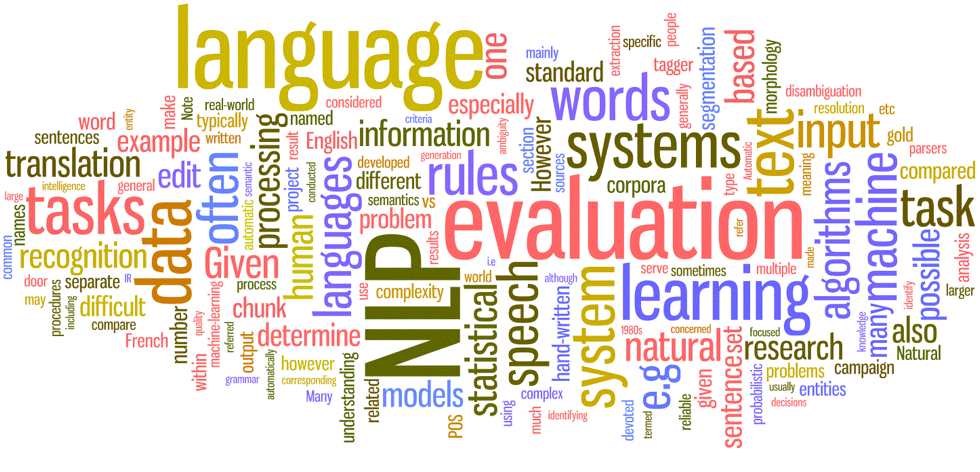
\includegraphics[width=7cm]{./figs/NLPTM_wordcloud.png}}

\end{frame}

%######################################################
%######################################################
\begin{frame}

	\frametitle{NLP challenges to machines}

	\large
	
	\begin{block}{Generic difficulties}
	\begin{itemize}
	
		\item Natural Language can be highly {\bf ambiguous}
		\item {\bf Disambiguation} of polysemic words
		\item {\bf Sentiment Analysis}
		\item {\bf Intention inference}: sarcasm, humor, etc
		\item Differentiate main from secondary topics
		\item Incorporate domain-expert knowledge into automatically inferred statistical models
	
	\end{itemize}
	\end{block}

	\begin{block}{Current challenging applications}
	\begin{itemize}
	
		\item Text summarization
		\item Automatic captioning
	
	\end{itemize}
	\end{block}


\end{frame}


%######################################################
%######################################################
\section{2. NLP components}

%######################################################
%######################################################
\begin{frame}

    \frametitle{Contents}

	\large

    \begin{enumerate}
  
    	\item What is Natural Language Processing?
    	\item {\bf \color{blue}{NLP components}}
    	\item NLP applications
    	\item NLP technological phases
    	\item Planning for the block
    
    \end{enumerate}

\end{frame}

%######################################################
%######################################################
\begin{frame}

	\frametitle{NLP levels}

    NLP systems usually require to integrate several components such as

	\begin{itemize}
		\item Written Text recognition
		\item Image or video feature extraction
		\item Speech transcription
		\item Speech generation (text-to-speech)
		\item Text processing
		\item Text representation
		\item Syntactic analysis
		\item Semantic Analysis
		\item Semantic Similarity evaluation

	\end{itemize}
	
\end{frame}


%######################################################
%######################################################
\begin{frame}

	\frametitle{Text Preprocessing and Document representation}

    Traditional Machine Learning methods are not well-suited to work with unstructured text
    \begin{itemize}
		\item Process text to fit ML requirements
		\begin{itemize}
		    \item Regular expressions
		    \item Tokenization
		    \item Part-of-Speech Tagging
		    \item Named Entity Recognition
		    \item Dependency Analysis
		    \item N-gram identification
		    \item Lemmatization
		    \item (Application specific) stopwords and equivalences
		    \item Word weighting
		\end{itemize}
	\end{itemize}
	\centerline{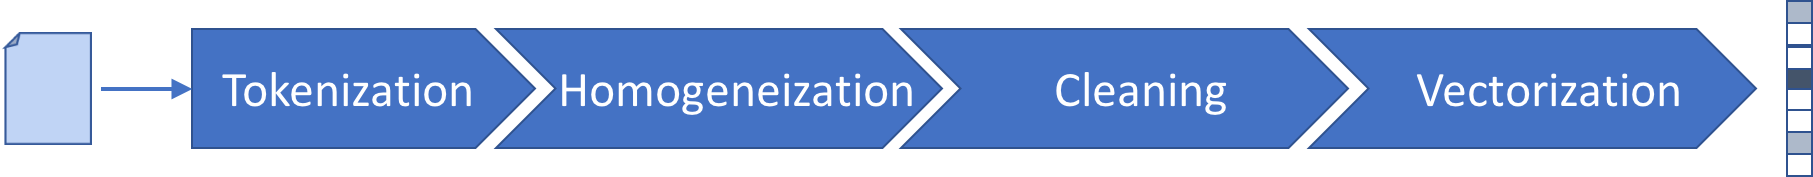
\includegraphics[width=11cm]{./figs/NLPTM_doc_preproc.png}}

\end{frame}

%######################################################
%######################################################
\begin{frame}

	\frametitle{Neural Networks for NLP}

    Traditional Machine Learning methods are not well-suited to work with unstructured text
    \begin{itemize}
        \item Develop novel ML structures that overcome these limitations
	\end{itemize}
    \centerline{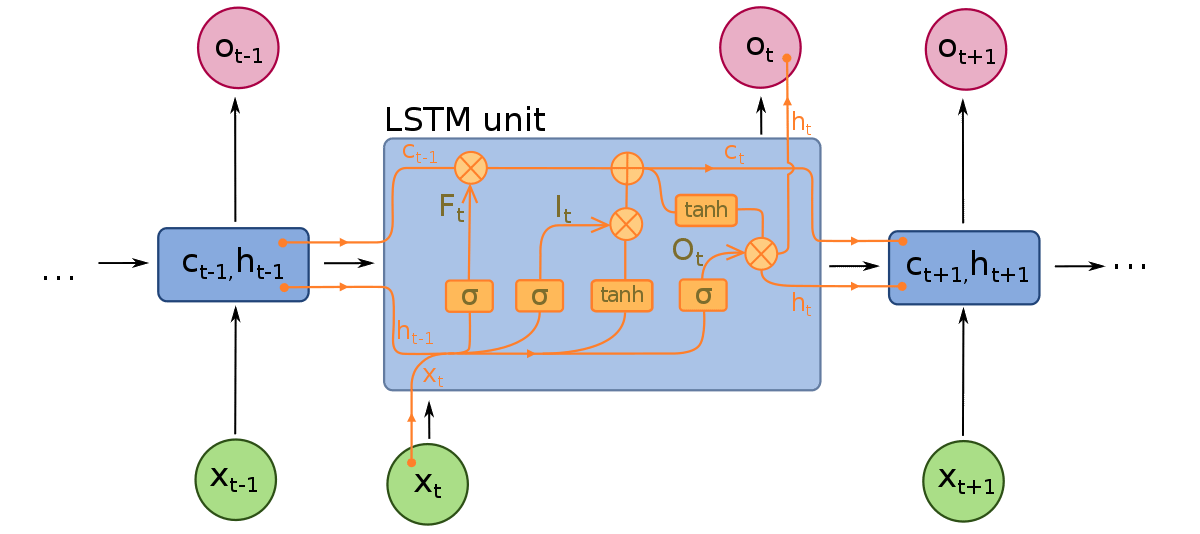
\includegraphics[width=9cm]{./figs/LSTM.png}}
    
    \footnotesize
	\begin{block}{Text Preprocessing vs NNs}
	\begin{itemize}
	
		\item Solid tools exist for both approaches
		\item Different applications require different solutions
	
	\end{itemize}
	\end{block}
	
\end{frame}

%######################################################
%######################################################
\section{3. NLP applications}

%######################################################
%######################################################
\begin{frame}

    \frametitle{Contents}

	\large

    \begin{enumerate}
  
    	\item What is Natural Language Processing?
    	\item NLP components
    	\item {\bf \color{blue}{NLP applications}}
    	\item NLP technological phases
    	\item Planning for the block
    
    \end{enumerate}

\end{frame}

%######################################################
%######################################################
\begin{frame}

	\frametitle{Machine Translation}

\centerline{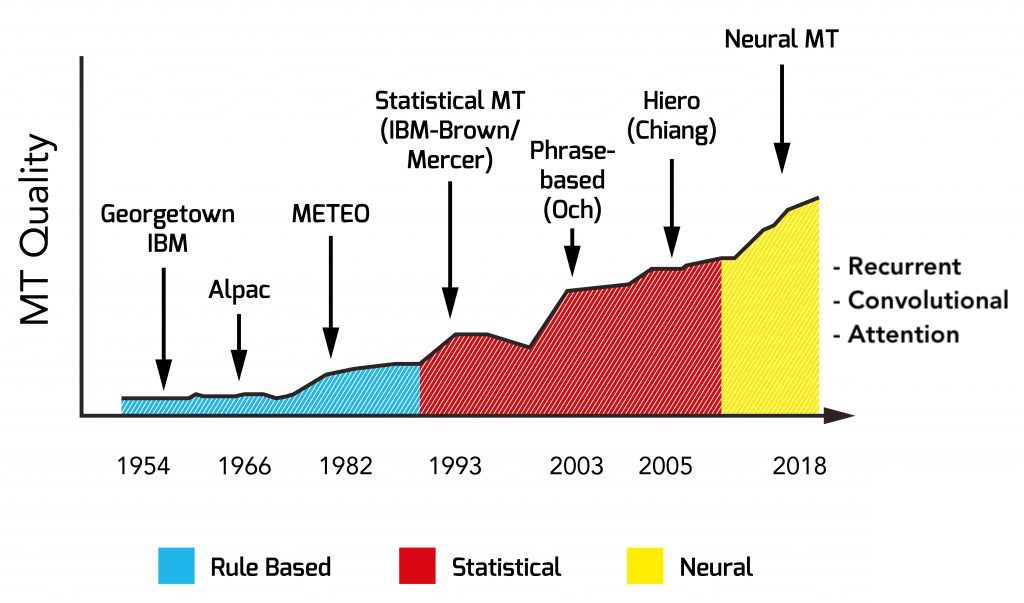
\includegraphics[width=12cm]{./figs/history_MT.jpg}}
\tiny
Source: IconicTranslation
(modified from https://nlp.stanford.edu/projects/nmt/Luong-Cho-Manning-NMT-ACL2016-v4.pdf)
\end{frame}

%######################################################
%######################################################
\begin{frame}

	\frametitle{Chatbots/Dialogue Systems}

\centerline{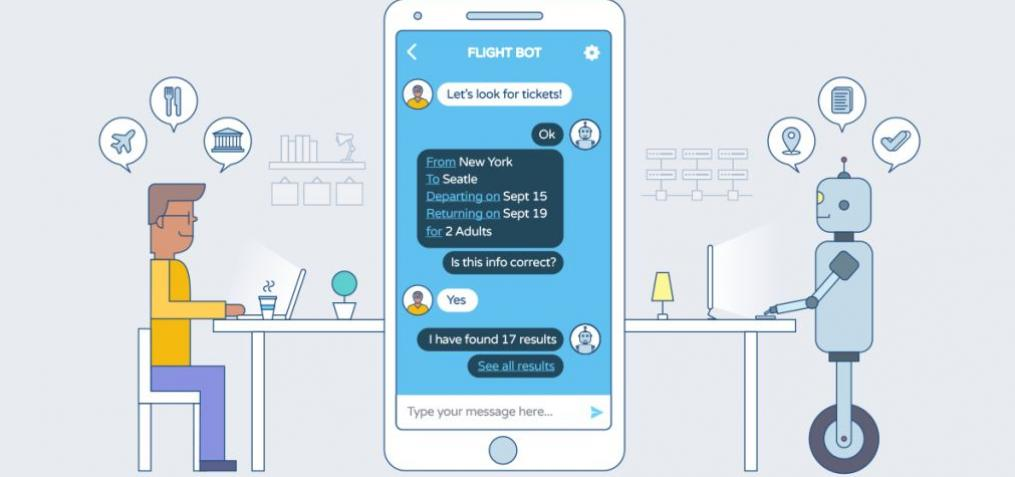
\includegraphics[width=12cm]{./figs/chatbot.jpg}}
\tiny
Source: https://vrroom.buzz/vr-news/tech/5-fantastic-examples-chatbots-apps
\end{frame}

%######################################################
%######################################################
\begin{frame}

	\frametitle{Sentiment Analysis}

\centerline{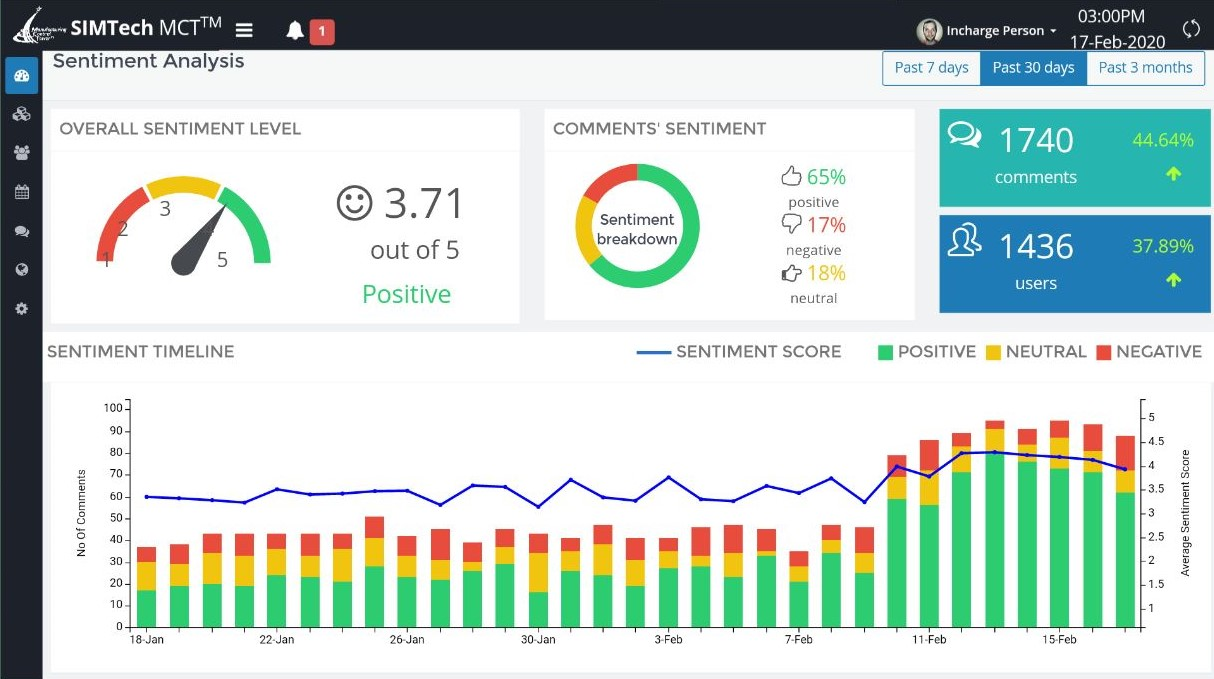
\includegraphics[width=12cm]{./figs/sentiment.jpg}}

\tiny
Source: Singapore Institute of Manufacturing Technology (SIMTech)

Free demo: \url{https://www.danielsoper.com/sentimentanalysis/default.aspx}
\end{frame}

%######################################################
%######################################################
\begin{frame}

	\frametitle{Topic Modeling}

\centerline{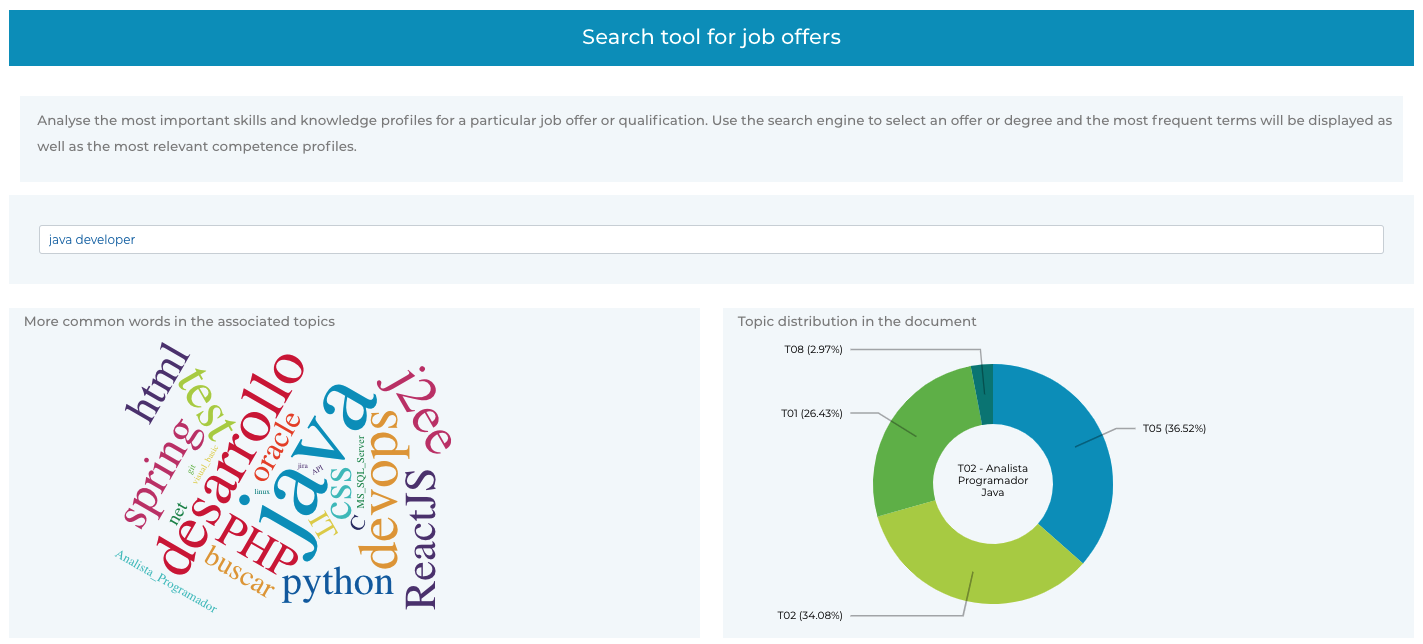
\includegraphics[width=12cm]{./figs/topic_modeling.png}}

\tiny
Source: \url{http://iad.ontsi.es/perfilestic2020/index.html}
\end{frame}

%######################################################
%######################################################
\begin{frame}

	\frametitle{Other applications}

\begin{itemize}
    \item Question answering
    \item Image/Video captioning
    \item Automatic subtitles
    \item Semantic search
    \item Predictive text
    \item Spelling and grammar checking
    \item Email filtering
    \item Competitive Intelligence
    \item Urgency detection
\end{itemize}
\end{frame}


%######################################################
%######################################################
\section{4. Technological phases}

%######################################################
%######################################################
\begin{frame}

    \frametitle{Contents}

	\large

    \begin{enumerate}
  
    	\item What is Natural Language Processing?
    	\item NLP components
    	\item NLP applications
    	\item {\bf \color{blue}{NLP technological phases}}
    	\item Planning for the block
    
    \end{enumerate}

\end{frame}



%######################################################
%######################################################
\begin{frame}

	\frametitle{Technological phases}

\vspace{.3cm}
\begin{itemize}
    \item 1960s: Formal grammars
    \begin{itemize}
        \item Finite number of symbols
        \item Languages are characterized by grammars with a finite set of rules
    \end{itemize}
\end{itemize}
\centerline{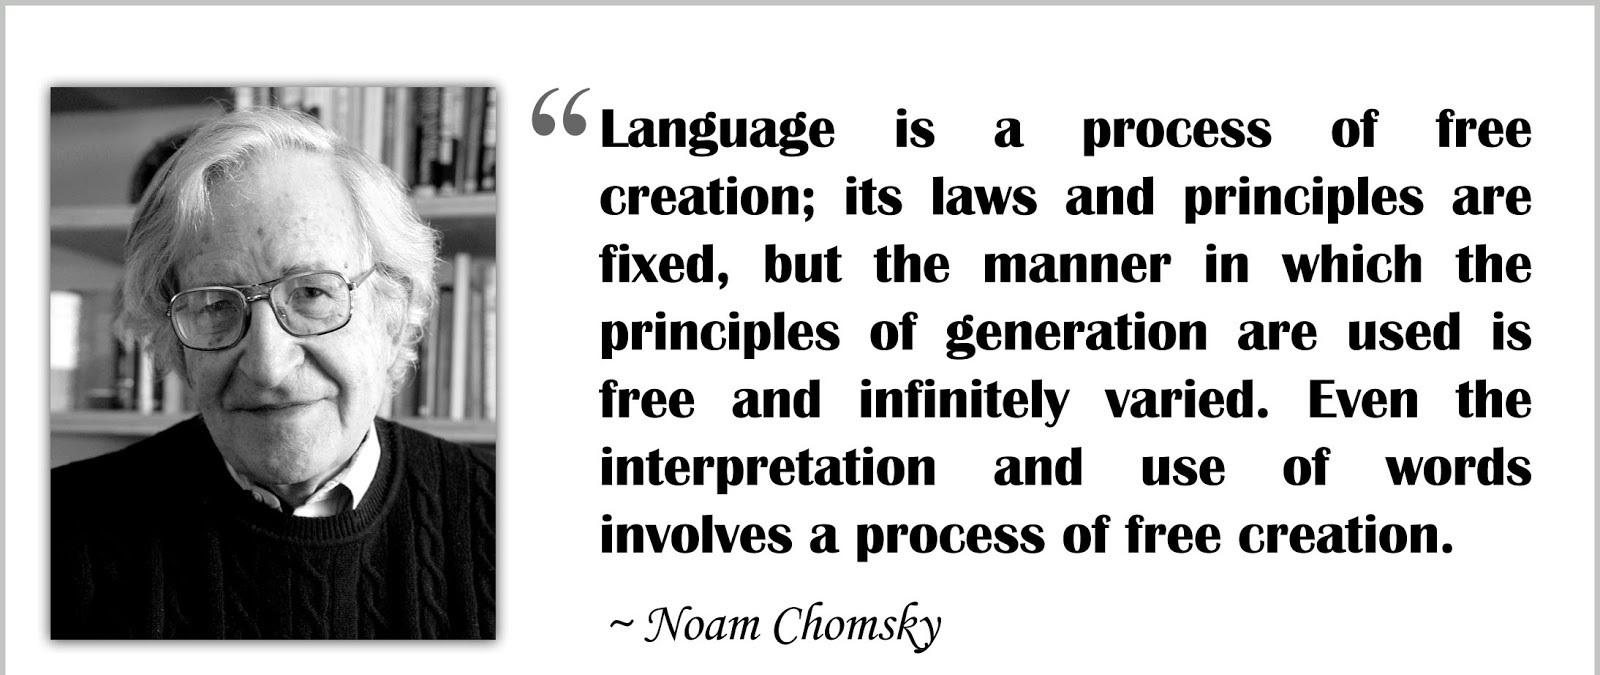
\includegraphics[width=10cm]{./figs/chomsky.jpg}}

\end{frame}

%######################################################
%######################################################
\begin{frame}

	\frametitle{Technological phases}

\vspace{.3cm}
\begin{itemize}
    \item 1990s: Computational linguistics
        \begin{itemize}
            \item Exploit statistical relations among words
            \item Annotated datasets for supervised learning tasks
        \end{itemize}

\end{itemize}
\centerline{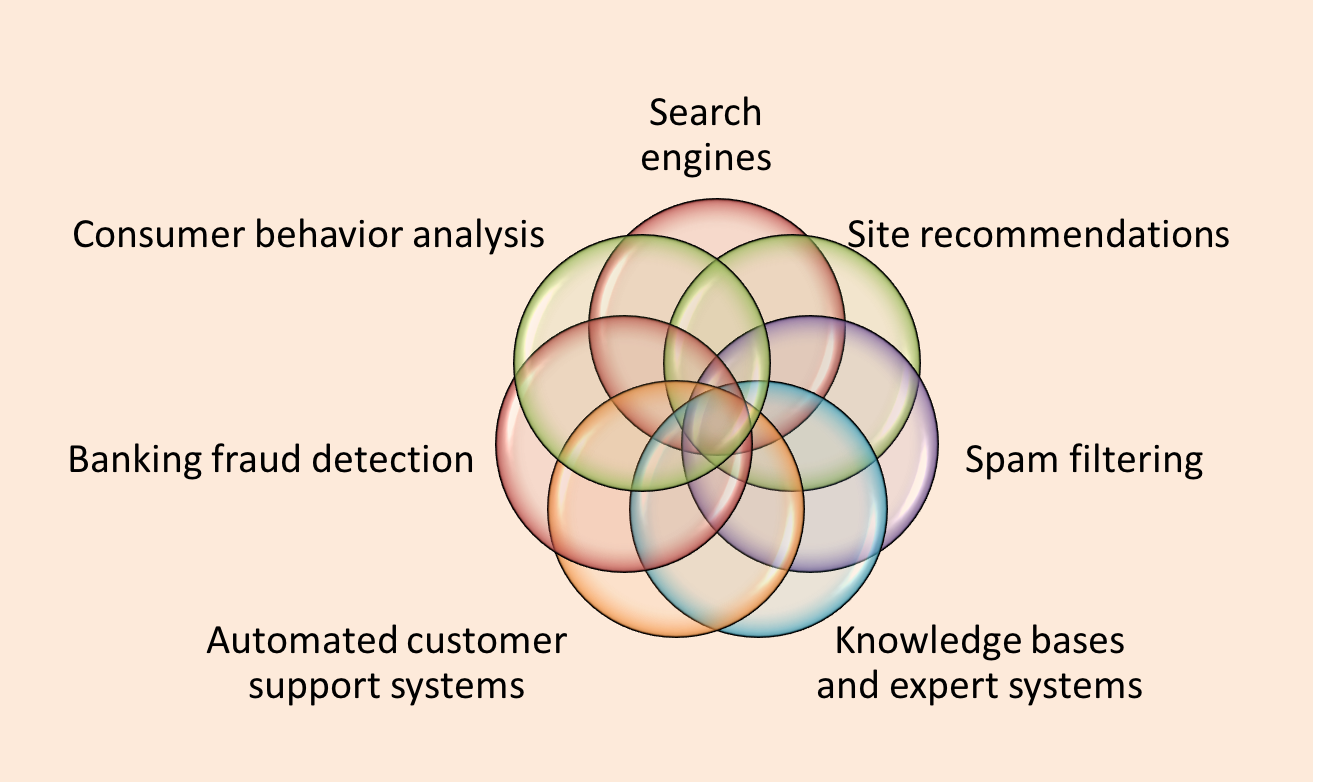
\includegraphics[width=10cm]{./figs/NLPTM_applications.png}}

\end{frame}


%######################################################
%######################################################
\begin{frame}

	\frametitle{Technological phases}

\vspace{.3cm}
\begin{itemize}
    \item 2010s: Deep learning
        \begin{itemize}
            \item Large amount of training data
            \item Transfer learning
            \item High-paralell and Cloud Computing
            \item Text-preprocessing generally not needed
            \item Lots of flexibility
        \end{itemize}

\end{itemize}
\centerline{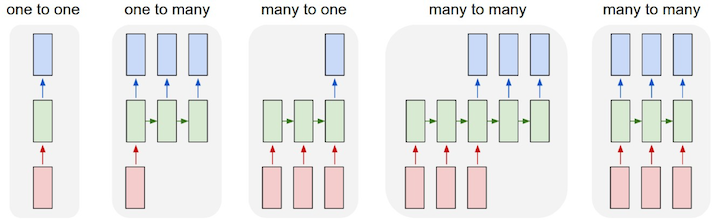
\includegraphics[width=10cm]{./figs/RNN_flexibility.png}}
\footnotesize
Image captioning / Sentiment Analysis / Machine Translation / Video captioning

\tiny
Source: \url{https://www.yuthon.com/post/tutorials/notes-for-cs231n-rnn/}
\end{frame}

%######################################################
%######################################################
\begin{frame}

\frametitle{NLP market}

\centerline{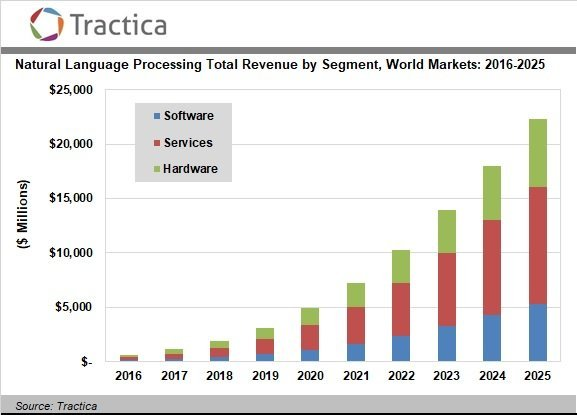
\includegraphics[width=10cm]{./figs/NLP_market.jpg}}

\tiny
Source: Tractica
\end{frame}

%######################################################
%######################################################
\begin{frame}

\frametitle{NLP market}

\centerline{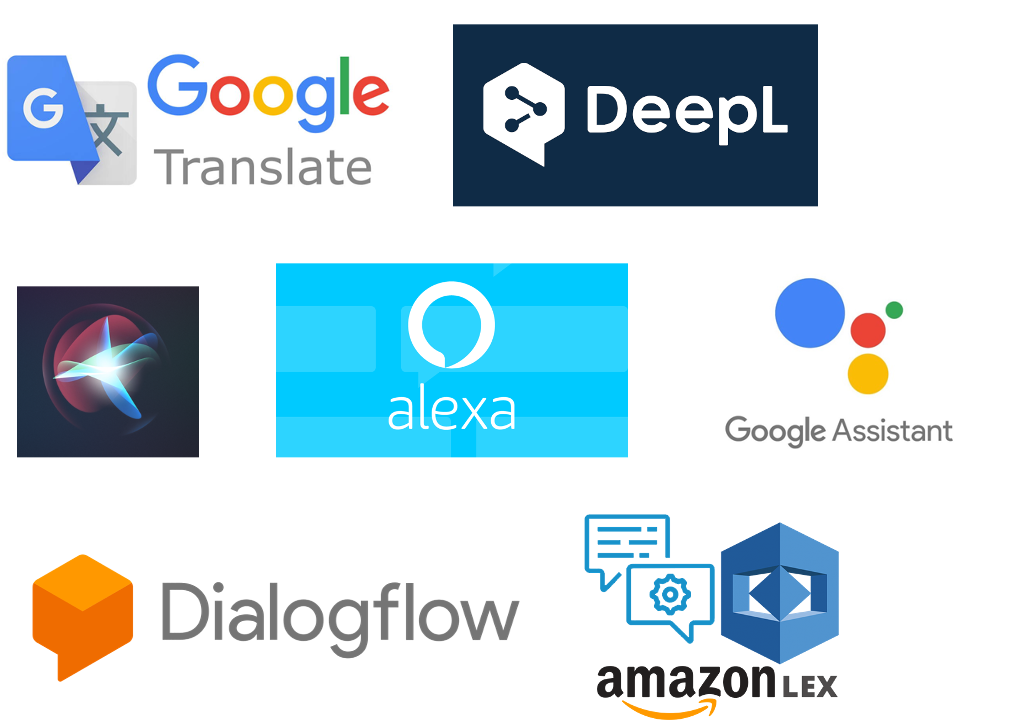
\includegraphics[width=10cm]{./figs/sota_companies.png}}
\end{frame}

%######################################################
%######################################################
\begin{frame}

\frametitle{Carbon emissions}

\centerline{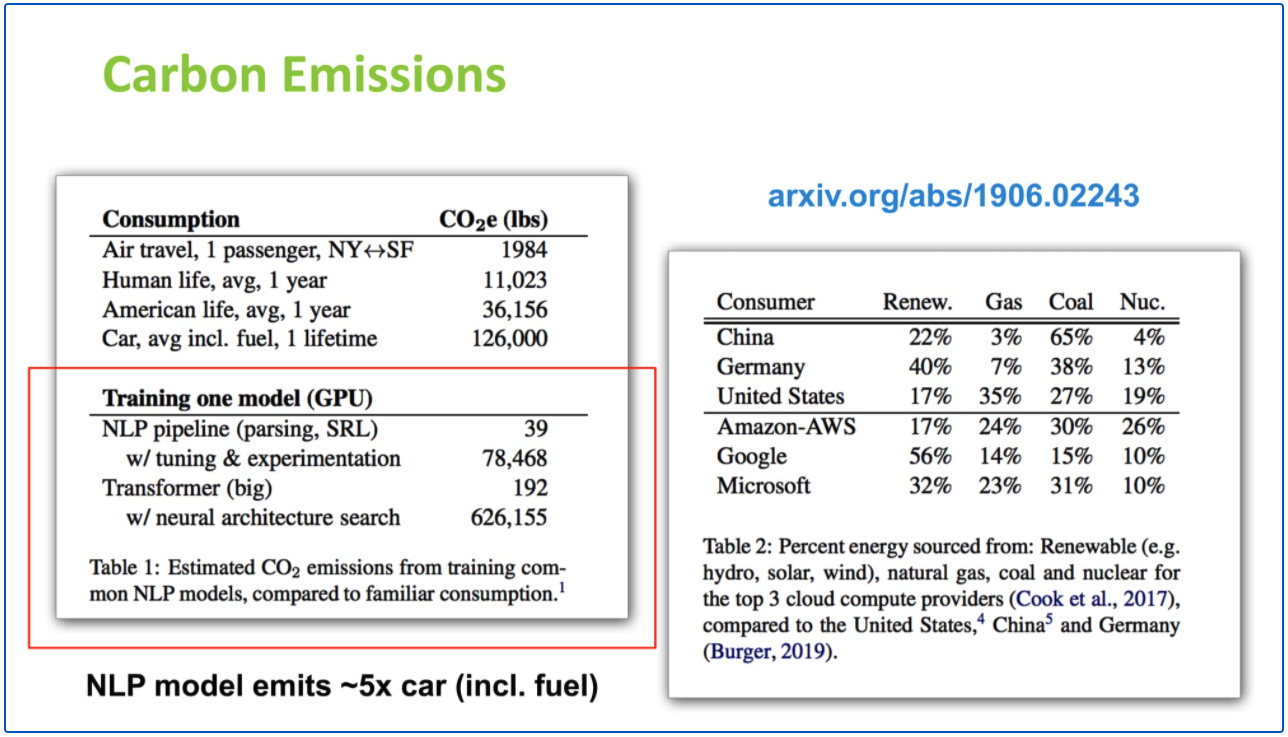
\includegraphics[width=10cm]{./figs/emissions.png}}

\tiny
Source: \url{https://derwen.ai/s/d5c7#55} (originally taken from arxiv.org/abs/1906.02243)
\end{frame}

%######################################################
%######################################################
\section{5. Block planning}

%######################################################
%######################################################
\begin{frame}

    \frametitle{Contents}

	\large

    \begin{enumerate}
  
    	\item What is Natural Language Processing?
    	\item NLP components
    	\item NLP applications
    	\item NLP technological phases
    	\item {\bf \color{blue}{Planning for the block}}
    
    \end{enumerate}

\end{frame}






%######################################################
%######################################################
\subsection{Block overview}

%######################################################
%######################################################
\begin{frame}

	\frametitle{Module overview}

We will implement a project covering an end-to-end implementation of an NLP system for document corpora topic modeling and analysis, including also visualization techniques.

	\begin{columns}
	
	\begin{column}{.3\textwidth}
		\vspace{.2cm}
		\centerline{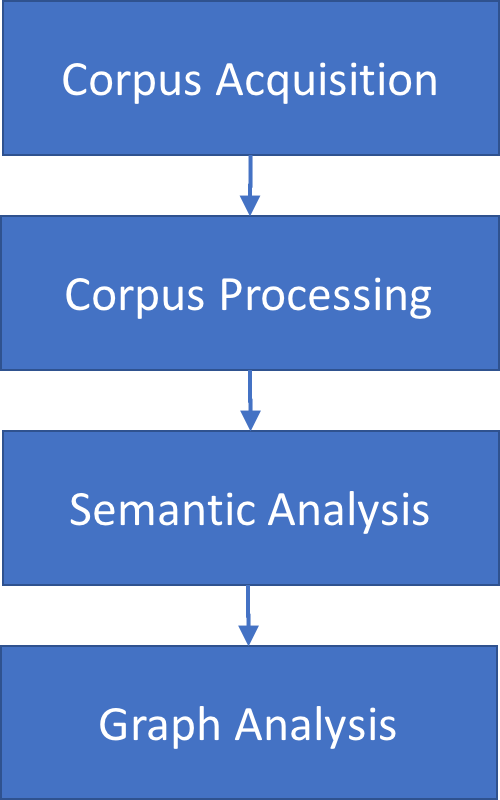
\includegraphics[width=.9\textwidth]{./figs/NLPTM_schema.png}}
	\end{column}
	
	\begin{column}{.6\textwidth}
		\begin{itemize}
			
			\item Discuss possibilities for corpus acquisition
			\item Present some of the most relevant text preprocessing techniques
			\item Present theoretical foundations and implementations of topic modeling algorithms
			\item Use the semantic representations to infer graphs among entities, and visualize them using Gephi	
			
		\end{itemize}
	\end{column}

	\end{columns}

\end{frame}

%######################################################
%######################################################
\begin{frame}

    \frametitle{Corpus Acquisition}

	There are many possibilities for acquiring interesting textual databases

	\begin{columns}
	
	\begin{column}{.5\textwidth}
		\begin{itemize}
			
			\item Web content (web pages, twitter, blogs, etc)
			\begin{itemize}
				\item Crawlers
				\item Available APIs (e.g., wikipedia, arXiv)
			\end{itemize}
			\item Local document collections
			\item Available corpus	
			
		\end{itemize}
	\end{column}
	
	\begin{column}{.5\textwidth}
		\vspace{.2cm}			\centerline{
\includegraphics[width=\textwidth]{./figs/NLPTM_wordcloud2.png}}
	\end{column}

	\end{columns}
	
Some applications examples
\begin{itemize}
\item Use job portals for modeling the job market in a country
\item Analyze innovation from patent descriptions
\item Categorize apps from their textual description in App stores
\item {\bf{Analyze public funding topics using projects abstracts}}
\end{itemize}

\end{frame}


%######################################################
%######################################################
\begin{frame}

	\frametitle{Tentative Plan for the NLP block}

\begin{tabular}{ll}Session 1 & Introduction to NLP. Corpus acquisition \\
\\
Sessions 2 \& 3 & Text preprocessing and document representation.\\
                & Spacy. Sentiment Analysis assignment. \\
\\
Sessions 4 \& 5 & Topic Modeling. Gensim. Mallet. \\
\\
Sessions 6 \& 7 & Semantic Similarity. Graph analysis. \\
                & Networkx, Gephi \\
\\
Sessions 8 \& 9 & Neural Language Models 
\end{tabular}

\end{frame}




\end{document} 